% Version 2020-01-06
% update – 161114 by Ken Arroyo Ohori: made spacing closer to Word template throughout, put proper quotes everywhere, removed spacing that could cause labels to be wrong, added non-breaking and inter-sentence spacing where applicable, removed explicit newlines
% update – 010819 by Dennis Wittich: made spacing and font size closer to Word template, updated references and refernces style
% update – 042319 by Dennis Wittich: font size of captions set to 'small', first author names are shortened, hyphenation fixed
% update – 010620 by Dennis Wittich: Footnotes alignment set to left

\documentclass{isprs} % isprs class modified 23-04-2019 (Dennis Wittich)
\usepackage{subfigure}
\usepackage{setspace}
\usepackage{geometry} % added 27-02-2014 Markus Englich
\usepackage{epstopdf}
\usepackage{natbib}
\usepackage{tabularx}
\usepackage{booktabs}
\usepackage[colorlinks, allcolors=blue]{hyperref}
%\bibliographystyle{apalike}
\usepackage[labelsep=period]{caption}  % added 14-04-2016 Markus Englich - Recommendation by Sebastian Brocks
\usepackage[british]{babel} 
\usepackage[hang]{footmisc}
%\setlength{\tabcolsep}{2pt}
\def\footnotemargin{1em} % added 08-01-2020 Dennis Wittich
\usepackage{fancyref}
\pagestyle{plain}

%\usepackage[authoryear]{natbib}
%\def\bibhang{0pt}

\geometry{a4paper, top=25mm, left=20mm, right=20mm, bottom=25mm, headsep=10mm, footskip=12mm} % added 27-02-2014 Markus Englich
%\usepackage{enumitem}

%\usepackage{isprs}
%\usepackage[perpage,para,symbol*]{footmisc}

%\renewcommand*{\thefootnote}{\fnsymbol{footnote}}
\captionsetup{justification=centering,font=normal} % thanks to Niclas Borlin 05-05-2016
\captionsetup[figure]{font=small} % added 23-04-2019 Dennis Wittich
\captionsetup[table]{font=small} % added 23-04-2019 Dennis Wittich

% Location of the images
\graphicspath{{figures/}}

\begin{document}

\title{Assessing Digital Elevation Models with different image overlap using photogrammetry}

% KAO: Remove extra spacing
\author{Robert van de Vlasakker\textsuperscript{a}}

% KAO: Remove extra newline
\address{
    \textsuperscript{a}
    Wageningen University \& Research} % Not needed

% If the corresponding author is NOT the final author, always add a % space before the subsequent comma, i.e.
% first author name\textsuperscript{a,}\thanks{Corresponding author} , % second author name \textsuperscript{b}, etc.
% thanks to Niclas Borlin 05-05-2016

% BB: leave these empty, but do not delete
\commission{}{} %This field is optional.
\workinggroup{} %This field is optional.
\icwg{}   %This field is optional.

% KAO: Use times symbol
\abstract{
Photogrammetry is easy to use these days and can be used to create a digital elevation models (DEM) of an area. 
Image overlap plays an important role in the process of photogrammetry.
A high overlap takes more time to gather in the field and takes longer to process.
Less overlap usually results in a less accurate calculations. 
In this paper the overlap of an area is artificially reduced and digital elevation models have been created with different image overlaps.
The DEM's are compared to see how reducing the image overlap influences the result. 
When the absolute values of the DEM are compared large differences are visible.
However, when the scaled DEM's are compared in a boxplot the differences appear to be minimal.
Finally, violin plots have been made of the complete image set DEM minus the reduces image set DEM's.
The more images are used, the more the difference of the DEM's is centered around 0.
The DEM of the dataset with the highest images count seems to be the most similar to the DEM of the full dataset.
}

\keywords{Photogrammetry, Digital Elevation Model, Image Overlap, Agisoft Metashape}

\maketitle

%\saythanks % added 28-02-2014 Markus Englich

\section{Introduction}\label{Introduction}

Photogrammetry is the process of reconstructing spatial information with images through computer vision. 
These days most photogrammetry data is acquired with unmanned aerial vehicles (UAV) \citep{UAVAreMoreUsed}. 
UAV's come with GNSS and provide high resolution images needed for photogrammetry.
The process uses similar points visible on multiple images to determine the points in 3D space.
The reconstruction certainty of these points is strongly dependent on the overlap between different images. 
A digital elevation model (DEM) is a popular product from photogrammetry \citep{DemIncrease1}.
A DEM is a 2D grid containing height values and is frequently used in geoinformation applications.
It is therefore important to create high quality DEM's.

A higher image overlap results in more similar image points, which will increase the reconstruction certainty of the points \citep{MoreOverMoreAcc}.
A higher image overlap, does not automatically results in a denser point cloud. \citep{EffectofUABimgcamover}. 
A high overlap is needed in complex structures like vegetation; if parts of the object are not visible on the image, they will not be reconstructed in the point cloud \citep{AccessingImageOverlap}.
However, an image dataset with a high overlap takes longer to gather, and may require multiple drone flights for a single dataset \citep{uavpop}.
In the reconstruction process, a high overlap will also result in longer computation time \citep{AccessingImageOverlap}
By reducing the image overlap, time and computing power may be saved without loosing too much spatial information.
%The goal of this study is to investigate the results on the image processing results of using reduced image sets of the same area. 
This main goal of this study is to investigate how different image overlap influences the DEM result that is created with photogrammetry.
It will be investigated how the different image overlap influence the intermediate photogrammetry results and processing time.





\section{Materials and Methods}

\subsection{Study Area}\label{sec:Study Area}
The data covers an area in Ghana, about 20km south east of Ejura (lat. 7.3064212, lon. -1.164493). 
The area of interest is about 25000 m\textsuperscript{2} and consists mostly of savanna area.
There are a few trees present on the observed location.
Each image has a resolution of 4000 times 3000 and was taken by a DJI Phantom 3.
The images all contain a GNNS location (WGS84). 
The complete data set consists of 111 images.
Their exact location can be found in figure \ref{fig:areaofinterest}.
\begin{figure}[h]
    \centering
    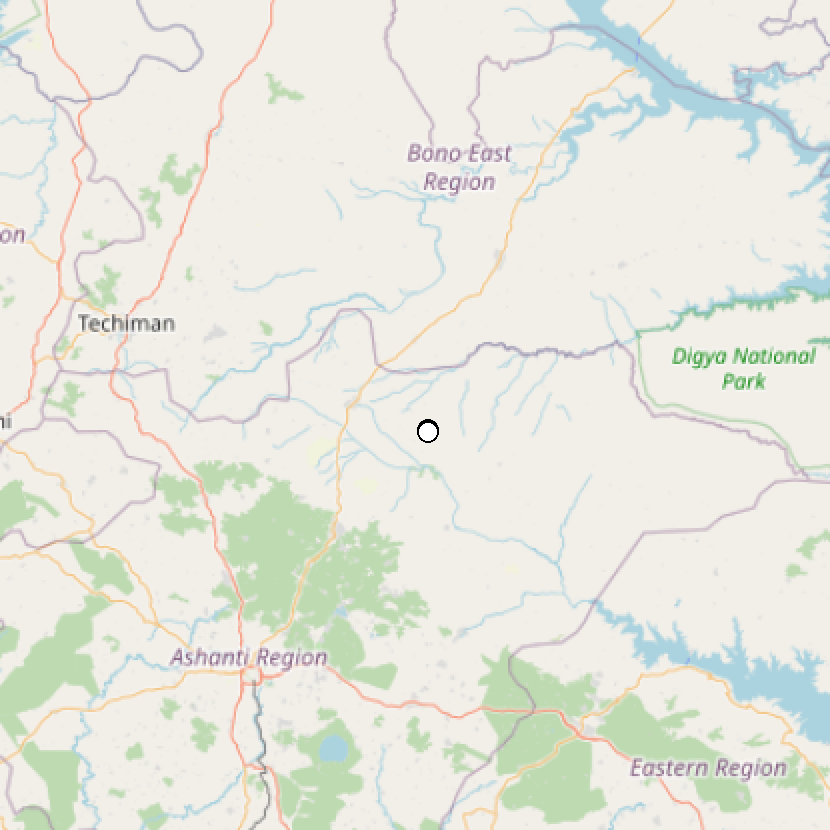
\includegraphics[width=4cm]{locationwide.png}
    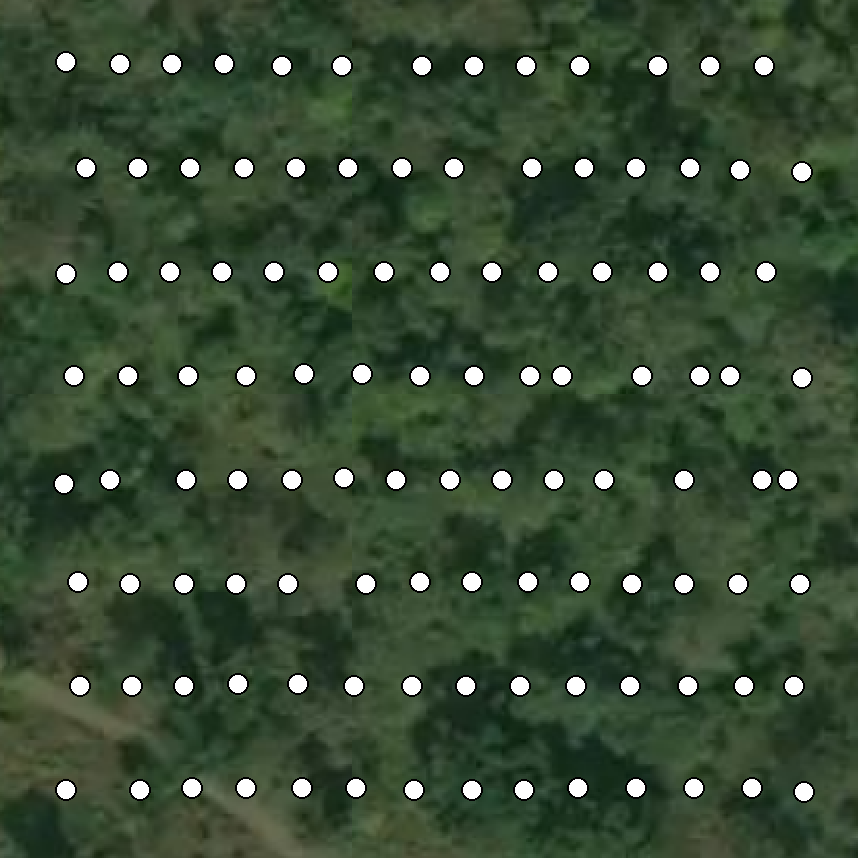
\includegraphics[width=4cm]{imgloc.png}
    \caption{Area of Interest and Unprocessed Image GPS Locations}
    \label{fig:areaofinterest}
\end{figure}


\subsection{Image Processing}
For image processing and DEM generation Agisoft Professional Edition 1.6.5 (Agisoft LLC., St. Peterburg, Russia) was used \citep{AgisoftMetashape}.
All data have been processed on the cloud service provided by Agisoft (\url{https://cloud.agisoft.com}).
The cloud processing is done on 32 vCPU's (Intel Xeon E5 2686 v4) with two NVIDIA Tesla M60 GPU's and 240 GB of RAM.

First, the complete data set has been aligned on medium quality.
On medium alignment quality the original images are scaled to have 1/2 of the original size.
%ADD MANUAL
Next, the dense cloud was built on medium quality (no depth filtering), resulting in a dense cloud of 3,268,264 points.
With medium settings the original photo is scaled to 1/4 before used in the dense cloud generation process.
%ADD MANUAL
A mesh was built using the the triangulated irregular network (TIN) algorithm by \citet{axelsson1999processing}. 
finally after the mesh, the Reduce Overlap function was used to reduce the amount images used in the process of photogrammetry. 
Because the final product of the photogrammetry process in this paper is a DEM a 2.5D height field was used when the mesh was generated
The 2.5D height field mesh contains only one Z value for any X, Y coordinate combination, this is also the case in the final DEM.

\textbf{Reduce Overlap.} 
The algorithm of the Reduce Overlap function tries to select a minimal amount of images such that each point of the model is observed from N locations/angles.
If a point is observed multiple times from the same location/angle, than this still counts as one. 
As in this research a height field was used, the algorithm will probably take the vegetation canopy into account in the reconstruction, but lower branches may be lost in the process.
This will have some influence on the Reduce Overlap setting; it becomes more flexible because single height values are used for each X, Y coordinate combination.
The algorithm and parameters behind the Agisoft Reduce Overlap function are proprietary software and therefore unfortunately unknown.
In Agisoft Metashape the Reduce Overlap had three different settings, low, medium and high. 
All of the settings are used and the remaining images are used for further processing.
The images are matched based on an adapted version of the SIFT algorithm \citep{lowe1999object, AgisoftMetashape}.
All the datasets are processed on medium settings for the image alignment.

\textbf{Dense Cloud.}
The result of the alignment of the images is used as input for the dense cloud generation.
The data has been processing on medium settings without any depth filtering for the generation of the dense cloud. 

\textbf{DEM.}
The source data for the DEM's are the dense cloud results. 
The TIN algorithm is used to built the DEM's \citep{axelsson1999processing}.
Because the dense clouds are unique the TIN algorithm also results in four unique DEM's.
These DEM's all have a slightly different extent and resolution.
For further comparison the DEM's have all been cropped on the largest common extent and the pixel resolution was set to 17.5 cm per pixel (1670 x 1290 pixels).
The DEM's were also be scaled to check the differences between the DEM's without looking at the absolute values.
The scaling was be done by subtracting the mean and dividing by the standard deviation.
For further comparison all of the DEM's were be subtracted from the full model DEM.
%%% CHECK THIS
These data will be used to inspect the differences between the scaled DEM of the full image dataset compared to the other DEM's.

\section{Results}
In table \ref{tab:ImageProcessing} the result of image processing for each Reduce Overlap settings can be found. 
The dense clouds contain about the same amount of points with the exception for the lowest Reduce Overlap setting, This setting has resulted in the dense cloud with the most points.

\begin{table}[h]
    \centering
    \caption{Image Processing Results}
    \begin{tabular}{@{}cccc@{}}
    \toprule
    \textbf{\begin{tabular}[c]{@{}c@{}}Reduce Overlap \\ Setting\end{tabular}} &
    \textbf{\begin{tabular}[c]{@{}c@{}}Image\\ Count\end{tabular}} &
    \textbf{Sparse  Cloud} &
    \textbf{Dense Cloud} \\ \midrule
    -      & 111 & 80,901 & 3,269,264 \\
    Low    & 44  & 37,886 & 4,172,783 \\
    Medium & 70  & 54,556 & 3,313,399 \\
    High   & 75  & 49,692 & 3,276,832 \\ \bottomrule
    % Add processing time!
    \label{tab:ImageProcessing}
\end{tabular}
\end{table}

For all the different datasets the processing time can be found in table \ref{tab:processingTime}.  

\begin{table}[h]
    \centering
    \caption{Processing time in seconds for the difference steps in the process.}
    \label{tab:processingTime}
    \begin{tabular}{@{}cccc@{}}
    \toprule
    \textbf{Image Count} & \textbf{Sparse  Cloud} & \textbf{Dense Cloud} & \textbf{Dem} \\ \midrule
    111                  & 150                    & 292                  & 17           \\
    44                   & 59                     & 443                  & 16           \\
    70                   & 83                     & 147                  & 17           \\
    75                   & 129                    & 159                  & 17           \\ \bottomrule
    \end{tabular}
\end{table}

After all the new datasets with the images have been aligned the camera locations are estimated, in figure \ref{fig:cameralocation} camera locations can be found. 
None of the images used in the alignment process failed to align.


\begin{figure}[h]
    \centering
    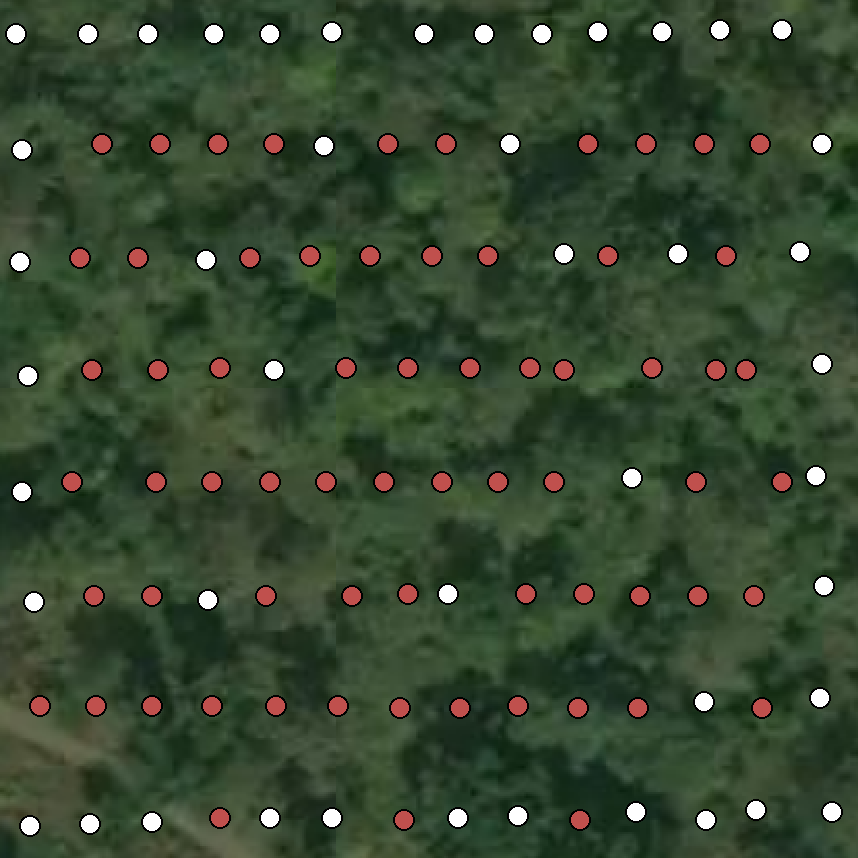
\includegraphics[width=1.9cm]{loc_low.png}
    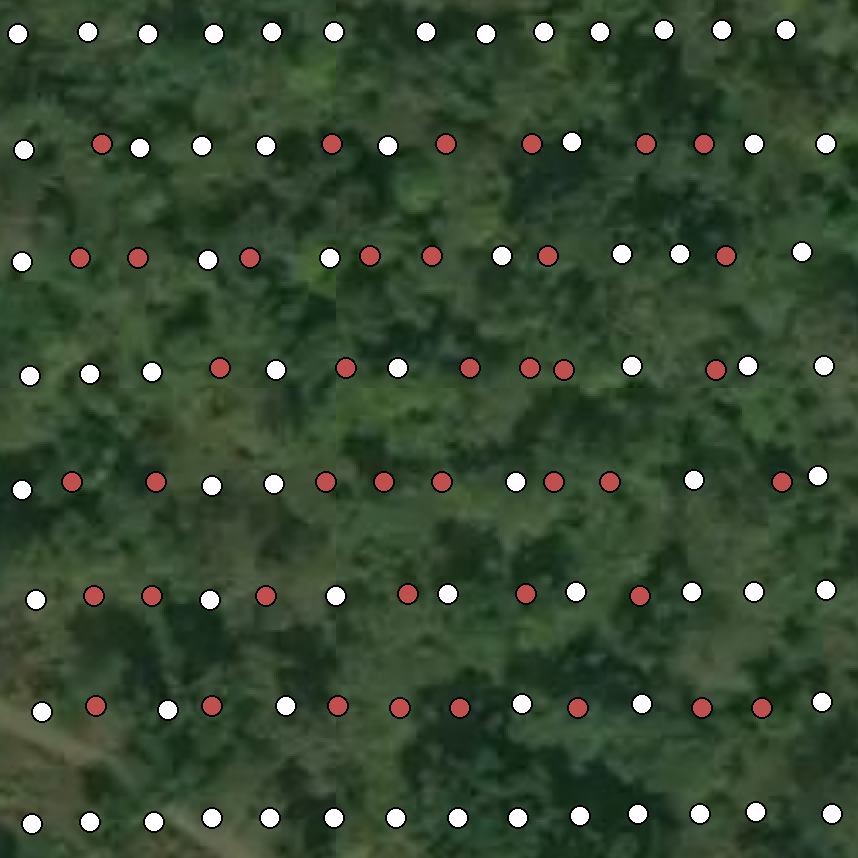
\includegraphics[width=1.9cm]{loc_med.png}
    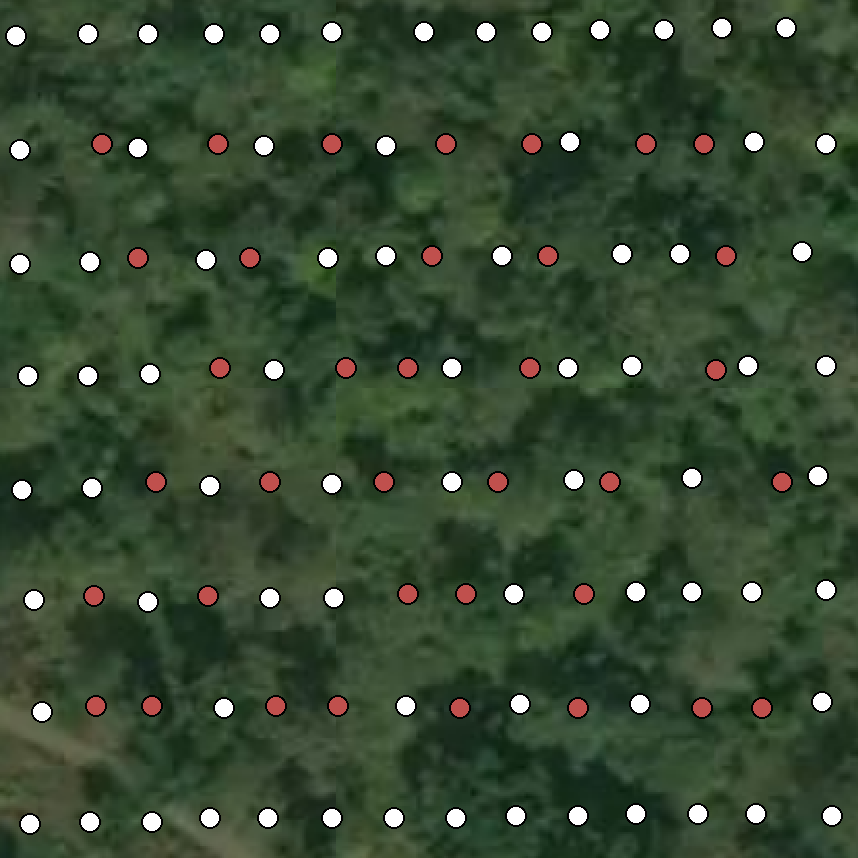
\includegraphics[width=1.9cm]{loc_high.png}
    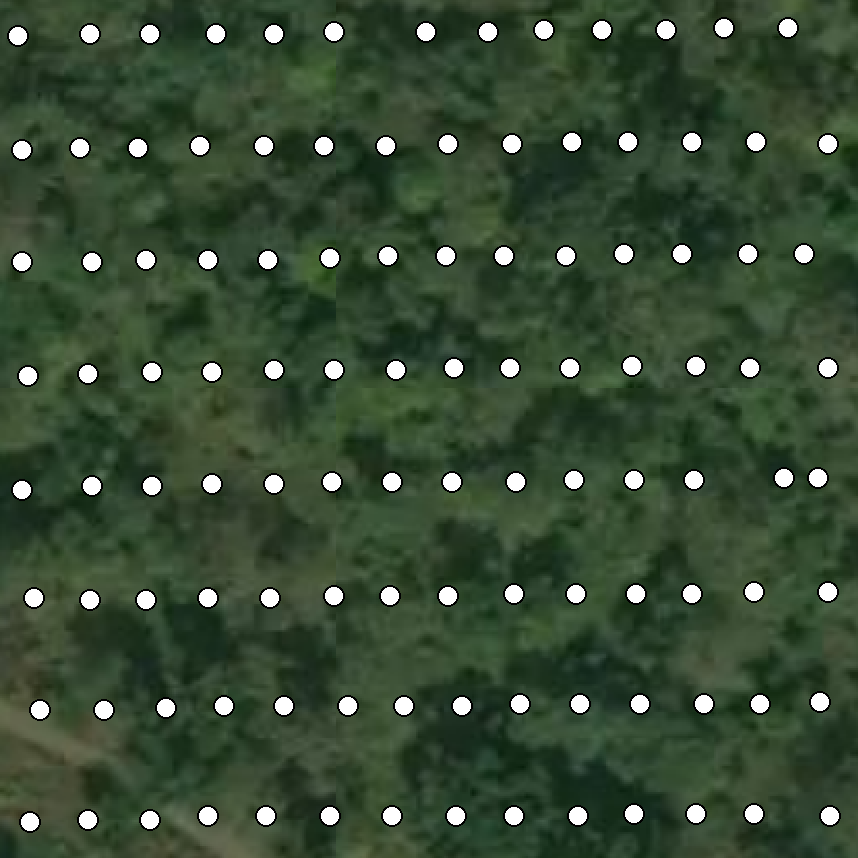
\includegraphics[width=1.9cm]{loc_full.png}
    \caption{Estimated camera location. 
    White: used in the image processing, red: disabled in the image processing.
    Starting left: low, medium, high and full settings}
    \label{fig:cameralocation}
\end{figure}

In figure \ref{fig:DemPlot_unscaled} the DEM's are visualized using the same color range. 
In this figure the DEM's do no look similar at all.

\begin{figure}[h]
    \centering
    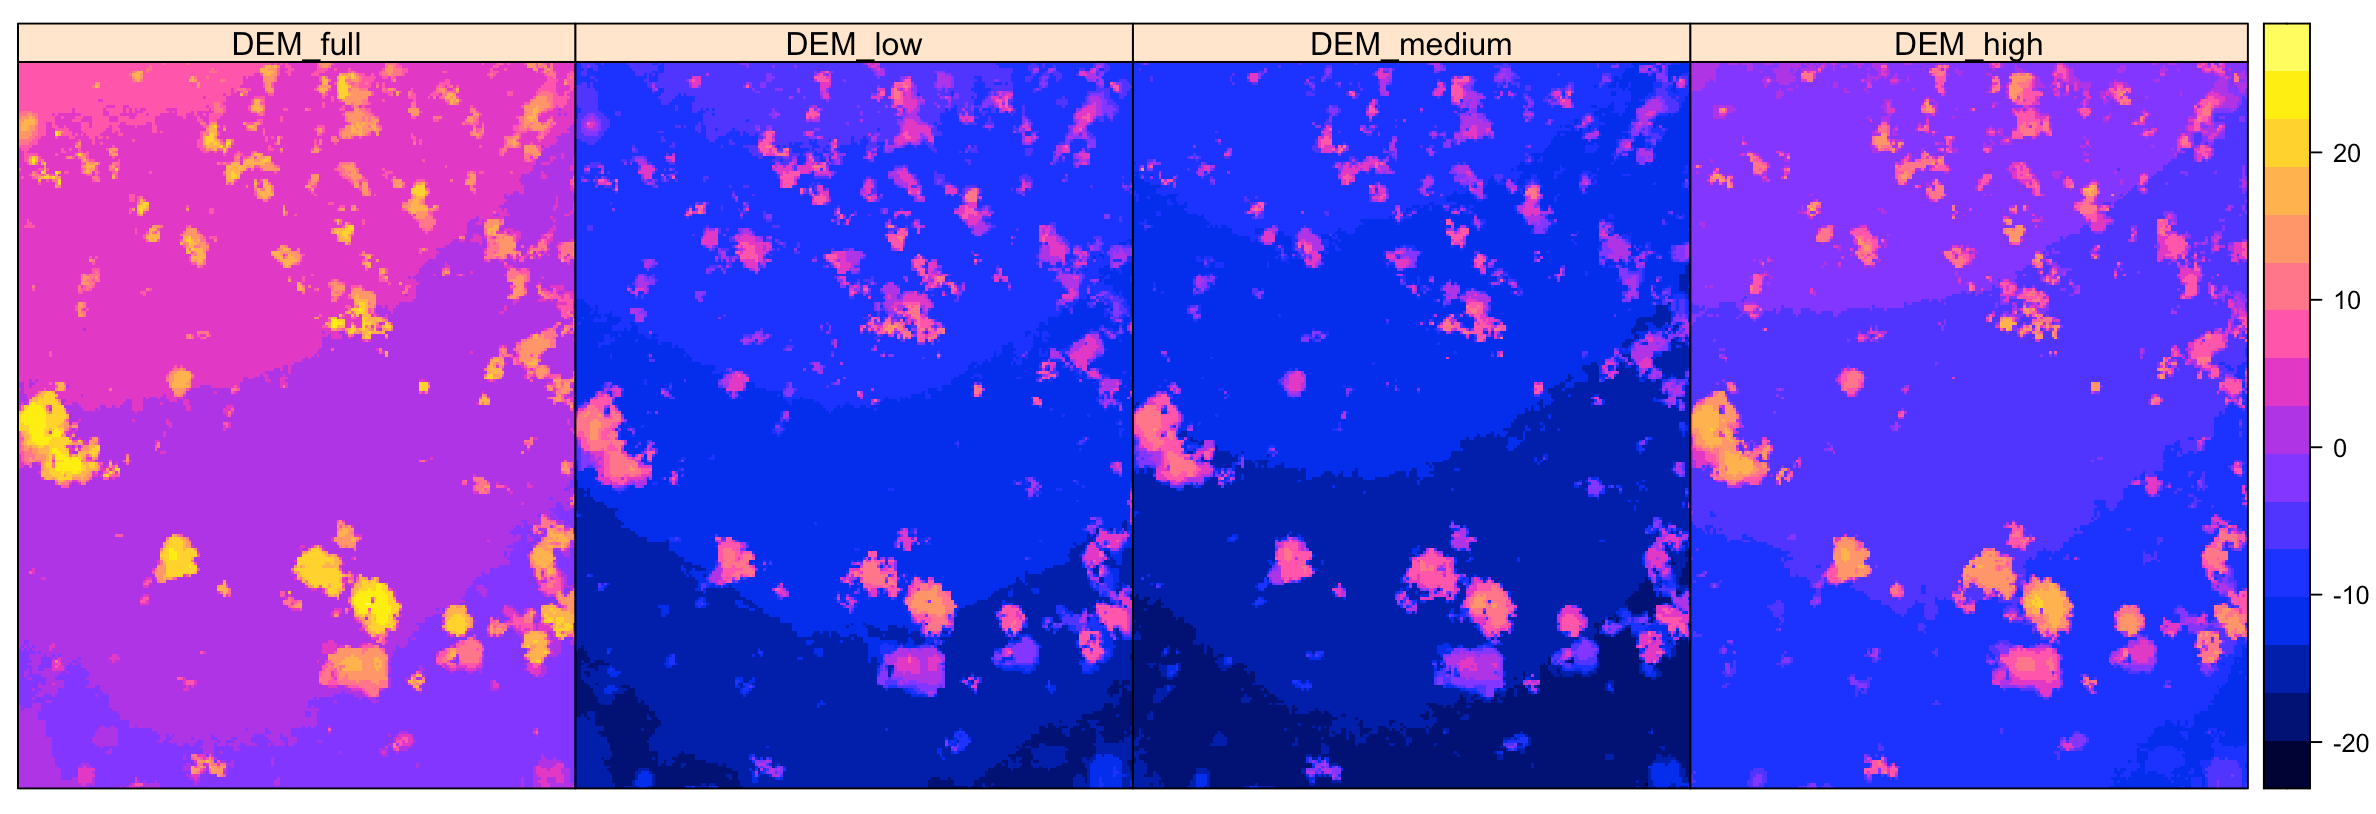
\includegraphics[width=8.5cm]{DemPlots.png}
    \caption{DEM Results of the Reduce Overlap}
    \label{fig:DemPlot_unscaled}
\end{figure}

As can be seen from figure \ref{fig:BoxPlot_unscaled} the DEM's are indeed different from each other. 
For the low setting the DEM values range from -19.4 to 19.0, for the medium setting the values range from -22.7 to 16.2, for the high setting the values range from 13.1 to 20.0 and for the full model from -4.8 to 28.9.

\begin{figure}[h!]
    \centering
    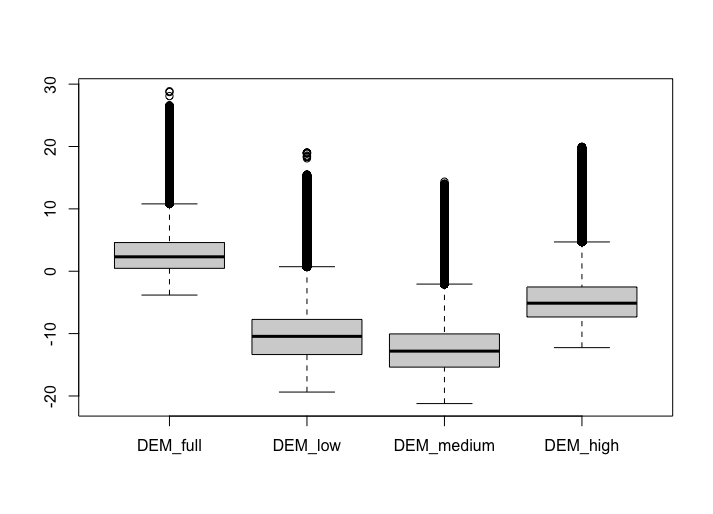
\includegraphics[width=8cm]{DemBoxplot.png}
    \caption{Box plots of the DEM Results of the Reduce Overlap}
    \label{fig:BoxPlot_unscaled}
\end{figure}

Figure \ref{fig:DemPlot_scaled} contains the same visualization of DEM plots, only for all the DEM's the data has been scaled.
There is almost no visual difference visible in the figure, the DEM's look quite similar.
This is confirmed in figure \ref{fig:BoxPlot_scaled}, only now the boxplot contain the scaled data values.
These difference seem to be minimal in the scaled boxplots.

\begin{figure}[h]
    \centering
    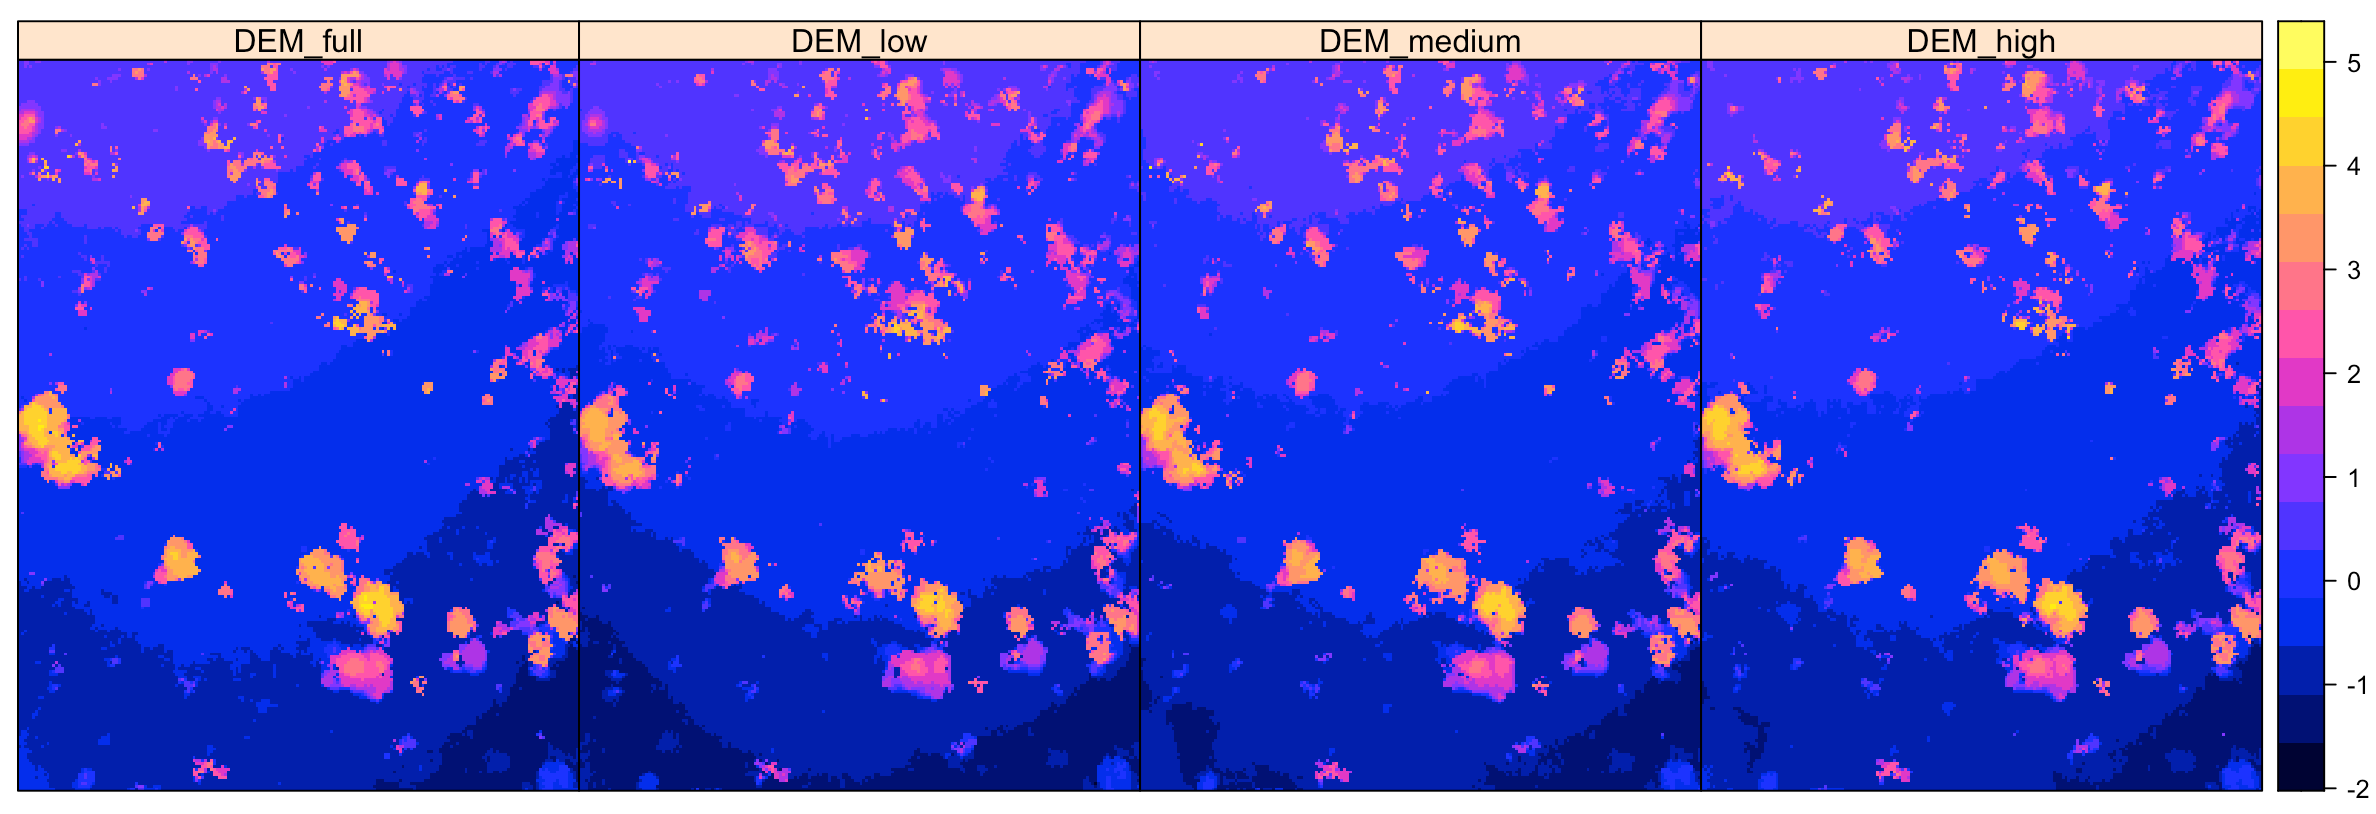
\includegraphics[width=8cm]{DemPlots_scaled.png}
    \caption{Scaled DEM Results of the Reduce Overlap}
    \label{fig:DemPlot_scaled}
\end{figure}



\begin{figure}[h]
    \centering
    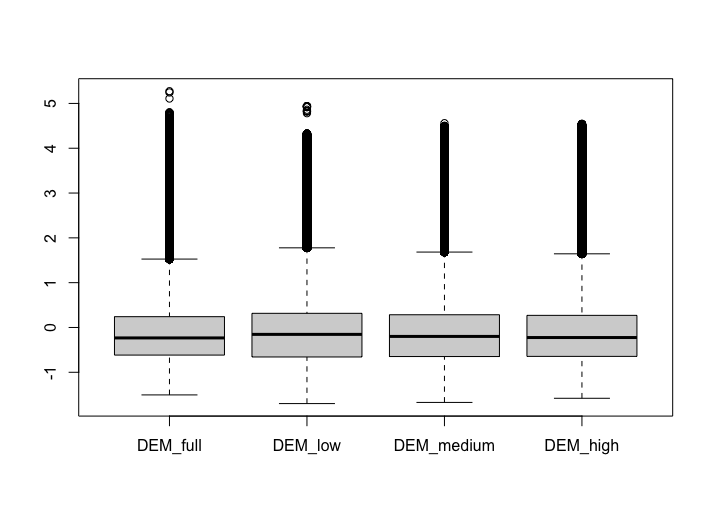
\includegraphics[width=8cm]{DemBoxPlot_Scaled.png}
    \caption{Scaled DEM Results of the Reduce Overlap}
    \label{fig:BoxPlot_scaled}
\end{figure}

Figure \ref{fig:ViolinPlot} contains three violin plots. For each of the plots the scaled DEM's from the reduced image datasets has been subtracted from the scaled full dataset DEM.
It is visible that the overall scaled error difference of the scaled DEM's varies from around -5.0 to 5.0.
For the high settings, the differences are more centered around zero, while this is not the case for low and medium settings.
For medium setting the difference is slightly more centered around 0.0 than low settings.

\begin{figure}[h]
    \centering
    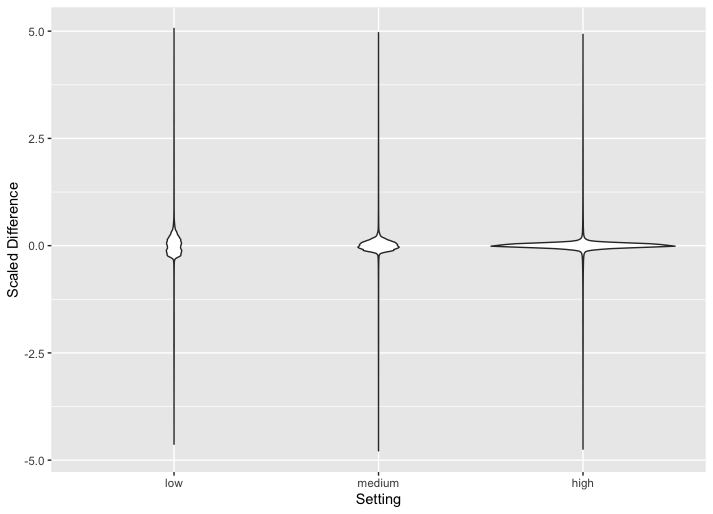
\includegraphics[width=8cm]{ViolinPlotOrdered.png}
    \caption{Violin plot of the difference between the full DEM and the reduced DEM's. All violin plots contain 2.154.300 measurements (1.670 rows x 1.290 columns)}
    \label{fig:ViolinPlot}
\end{figure}


\section{Discussion}
The goal of this research was to assess the difference between DEM's of the same area with different image overlap. 
The image reduction in the paper was calculated in Agisoft Metashape with the Reduce Overlap function.
The amount of images used in the processing does not seem to influence the density of the dense cloud, which was also concluded by \citet{EffectofUABimgcamover}.
In this research the point confidence was not measured, the dense cloud were directly used to construct a DEM. 

%The input mesh for the Reduce Overlap was a 2.5D height field. 
%This could be of influence, because the 2.5D mesh only takes one single height value into account for each %X, Y combination. 

%With more complex objects that need to processed as a real 3D object the quality of dense cloud may decrease if the amount of images is reduces significantly.
%Because the mesh was structured as a 2.5D surface, difficult points were removed from the model, e.g. in this case the tree canopies were constructed, but e.g. lower branches were lost in the construction process.
%An other option is that the Reduce Overlap function will not have much influence on the image count.

There is a large different between the absolute values between the different DEM's, this can be seen visually in figure \ref{fig:DemPlot_unscaled} and also when comparing the boxplot values in figure \ref{fig:BoxPlot_unscaled}.
The outliers in both boxplot figures are probably the vegetation that is present in the area as the boxplots only contain high outliers.
With the use of at least three ground control points the error in the absolute values of the can be reduced \citep{AssessingUAVGCPS, GCPbetterAccuracy, GeoreferencedPointClouds}.
Using GCP's in the different image dataset will reduce the absolute error.

The violin plots indicate that the dataset with the highest image count is most similar to the full dataset; the difference of is more centered around zero, while the two lower image count datasets are more widespread.
The largest errors differences (around -5/5) between the scaled DEM seem to be the same for all the image datasets.
The modelling software probably has difficulties in modelling the complex structures of the vegetation, resulting in a larger difference when the image count is lower.
This could result in more error around vegetation canopies where the algorithm has difficulties in accurately measuring the height. 
\citet{AccessingImageOverlap} also concluded that for complex structures a higher image overlap provides better results.
An other option may changing the filtering setting provided by the Metashape dense cloud generation.
In this research no depth filtering was used, by applying a more aggressive filtering technique the complex structures of the vegetation will be lost in the DEM generation \citep{AgisoftMetashape}.
Further research is needed to see where this differences exactly occur and if a different depth filtering may result in different results.

\section{Conclusion}
Using different image overlap in the same area results in DEM's with different absolute values.
The two image dataset with the least images show the largest difference in absolute value range compared to the original dataset with all images. 
The image dataset with the highest image count, has a DEM that is most similar compared to the original dataset.
When the scaled values are compared there seems to be a minimal difference between the DEM's.
If more images are used in the dataset, the difference between the scaled DEM's compared to the full images set becomes smaller; the DEM differences are more centered around 0.


% KAO: Sloppy spacing ensures non-overfull lines. Can be removed if this is not an issue.
\sloppy




{
	\begin{spacing}{1.17}
		\normalsize
		\bibliography{bibliography} % Include your own bibliography (*.bib), style is given in isprs.cls
	\end{spacing}
}



\vspace{1cm}
\end{document}





Photogrammetry is the process of reconstructing spatial information with images through computer vision. 
The process uses similar points visible on multiple images to determine the points in 3D space.
The reconstruction certainty of these points is strongly dependent on the overlap between different images. 
When a point is visible on more images, the reconstruction certainty will be higher \citep{MoreOverMoreAcc}.
This is especially the case with the reconstruction of irregular formed object like vegetation \citep{AccessingImageOverlap}.
With irregular objects, a higher overlap is preferred to capture each side of the object.
If parts of the object are not visible on the image, they will not be reconstructed in the point cloud.
In the reconstruction process, a high overlap will also result in longer computation time \citep{AccessingImageOverlap}
However, a higher image overlap, does not automatically results in a denser point cloud. \citep{EffectofUABimgcamover}. 
These days most photogrammetry data is acquired with Unmanned Aerial Vehicles (UAV) \citet{UAVAreMoreUsed}. 
UAV's come with high resolution cameras, GNSS and are available almost anywhere these days.
While UAV's do come with high resolution sensors and are relatively cheap, small, high capacity batteries are not available \citep{UAVpopularity}.
A high image overlap takes longer to gather than a low image overlap. 
A drone can use a higher altitude so the sensor captures a larger area.
however, with a higher flight altitude the detail of the image will be less than that of a drone with a lower flight altitude.
This way the gathering process takes longer, and the UAV might even need to switch batteries instead of taking the images in a single flight.
By reducing the image overlap, time and computing power may be saved without loosing too much spatial information.
This main goal of this study is to investigate how different image overlap influence the DEM result that is created with photogrammetry. 